% Drawing 156-8/04-1 -- folder 156-8, batch 04, archive page 80 (PDF page 81).
% Transcription: En marge gauche, en bas : un fuseau hachuré, entre deux points, coupé par un segment ; légendes $|B|$, $|A|$, « $A \cap B = \emptyset$ », « $|A| \cap |B| \neq \emptyset$ ». Il illustre deux parties disjointes dont les supports se rencontrent.
% Kind: plane figure (hatched lens, segment). Method 2 (schematic redraw from the facsimile). Status: ok.
% Notes: A hatched spindle between two points, crossed by a segment with a marked point; legends |B|, |A|, A cap B = empty, |A| cap |B| != empty. The marginal text written slantwise around it belongs to the transcription.
% Coordinates: 1 unit = 1 mm = 1/100 of the crop width (bbox in page fractions: [0.07, 0.5, 0.31, 0.77]).
% Redrawn by Claude (claude-opus-5-5), issue #73 pilot, 2026-11-07; not checked by a human; not compiled (no TeX in the session).
% Rights: reproduces part of the work -- behind RENDER_TRANSCRIPTS, never published by itself.
\documentclass[tikz,border=3pt]{standalone}
\usepackage{amsmath,amssymb}
\usetikzlibrary{patterns,arrows.meta}
\tikzset{pencil/.style={black!45}, struck/.style={black!35}, mark/.style={circle,draw,inner sep=1.3pt}, pt/.style={circle,fill,inner sep=0.9pt}, opt/.style={circle,draw,fill=white,inner sep=1.1pt}}
\begin{document}
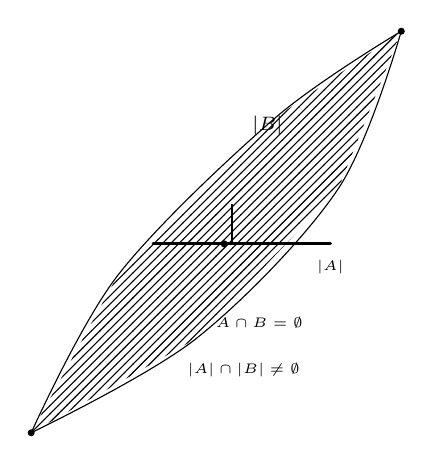
\begin{tikzpicture}[x=1mm,y=1mm,line cap=round,line join=round,font=\scriptsize]
\fill[pattern=north east lines] (19,-121) -- (30,-101) -- (50,-81) -- (66,-70) -- (58,-90) -- (40,-109) -- cycle;
\draw plot[smooth, tension=0.55] coordinates {(19,-121) (30,-101) (50,-81) (66,-70)};
\draw plot[smooth, tension=0.55] coordinates {(19,-121) (40,-109) (58,-90) (66,-70)};
\node[pt] at (19,-121) {};
\node[pt] at (66,-70) {};
\draw[very thick] (34.5,-97) -- (57,-97);
\node[pt] at (43.5,-97) {};
\draw (44.5,-92) -- (44.5,-97);
\node[inner sep=1pt] at (49,-82) {\scriptsize $|B|$};
\node[inner sep=1pt] at (57,-100) {\tiny $|A|$};
\node[inner sep=1pt] at (48,-107) {\tiny $A\cap B=\emptyset$};
\node[inner sep=1pt] at (46,-113) {\tiny $|A|\cap|B|\neq\emptyset$};
\end{tikzpicture}
\end{document}
